% !TEX TS-program = pdflatex
% Unbundling LLM Recommenders: Retrieval, Expression, and Consumer Choice
% Working draft for QME conference, May 15 2026.
%
% Style anchors:
%  - Structure: Gui and Kim (2025).
%  - Econometric expression: Feldman, Venugopal, Spiess, and Feder (2026).
%  - Voice: prior work by the author (Twitch gambling-ban paper).

\documentclass[11pt]{article}
\usepackage[margin=1in]{geometry}
\usepackage{amsmath, amssymb, amsthm}
\usepackage{microtype}
\usepackage{booktabs}
\usepackage{graphicx}
\usepackage{caption}
\usepackage{hyperref}
\usepackage[round]{natbib}
\usepackage{enumitem}
\usepackage{xcolor}
\usepackage{stackengine}
\usepackage{setspace}
\hypersetup{colorlinks=true, linkcolor=blue!50!black, citecolor=blue!50!black}
\onehalfspacing

\newtheorem{assumption}{Assumption}
\newtheorem{remark}{Remark}
\newtheorem{result}{Result}

\newcommand{\Real}{\mathbb{R}}
\newcommand{\Expect}{\mathbb{E}}
\newcommand{\E}{E}
\newcommand{\J}{J}
\newcommand{\Y}{Y}
\newcommand{\X}{X}
\newcommand{\Q}{Q}
\newcommand{\Z}{Z}
\newcommand{\Qreg}{D^J}
\newcommand{\Rreg}{D^T}
\newcommand{\catalog}{\mathcal{A}}
\newcommand{\dR}{\Delta_J}
\newcommand{\dP}{\Delta_T}
\newcommand{\dRP}{\Delta_{JT}}
\newcommand{\dtotal}{\tau^{BB}}
\newcommand{\KOS}{K^{BB}}
\newcommand{\KMO}{K^{MO}}
\newcommand{\genneq}{\stackrel{\textit{\scriptsize generally}}{\neq}}

\title{\textbf{Unbundling LLM Recommenders:\\ Retrieval, Expression, and Consumer Choice}}
\author{Qifan Han\thanks{Chinese University of Hong Kong, Shenzhen. Email: \href{mailto:hanqifan@cuhk.edu.cn}{hanqifan@cuhk.edu.cn}}}
\date{This draft: \today}

\begin{document}
\maketitle

\begin{abstract}
\noindent
When an LLM shopping assistant improves consumer outcomes, is the gain driven by better product selection or by more effective recommendation language? Standard A/B tests of LLM recommenders identify the total effect of a policy change, but they leave the product-selection and expression channels bundled. This paper proposes a modular experimental design that crosses a retrieval policy with an expression policy in a factorial structure, separately estimating retrieval, expression, and interaction effects as deployable firm interventions. In a semi-synthetic study with 30 real headphone products from Amazon and 60 consumer personas, we apply a history-access shock---whether the recommender observes historical marketplace metadata and buyer feedback---to each stage independently. In this setting, GPT-based synthetic evaluation shows two large, opposing effects that a bundled test would miss: routing historical information to product selection reduces evaluated recommendation quality through premium-aspiration bias, while routing the same information to text generation improves trust and tradeoff disclosure. The best-performing configuration is a hybrid that no bundled test can observe. We also show that regressions using realized expression intensity can overstate the language channel when expression covaries with latent product-consumer fit. The framework offers e-commerce platforms and marketing technology firms a practical tool for diagnosing which layer of an LLM recommendation pipeline creates value.
\end{abstract}

\medskip
\noindent\textbf{Keywords:} AI shopping assistants, product recommendation, causal decomposition, consumer choice, digital marketing experimentation.

\bigskip
%-------------------------------------------------------------------------
\section{Introduction}
%-------------------------------------------------------------------------

AI agents are becoming a new shopping interface on e-commerce platforms, guiding consumers through product discovery, comparison, and choice with backend support from large language models (LLMs). We refer to these systems as LLM recommenders: shopping assistants that use an LLM to select products and generate consumer-facing recommendation text. A consumer can ask for a laptop for graduate school, headphones for air travel, or a charger for multiple devices, and receive a conversational recommendation rather than a ranked product list. This interface differs from conventional search and recommendation in one important respect: the assistant does not only decide \emph{what} product to show. It also generates the language that explains, frames, and justifies the recommendation. The product and the explanation arrive as a single generated recommendation package.

This bundling creates a new measurement problem for firms. Suppose a retailer changes the backend instruction, retrieval source, or historical-information access of an LLM shopping assistant and observes a higher click or purchase rate. A standard randomized prompt or policy A/B test identifies the total effect of that change. But the total effect is not enough to answer the next managerial question. Did the new policy help because the assistant selected better products? Did it help because the assistant wrote more credible or persuasive recommendation text? Or did it help only when a particular product-selection rule was paired with a particular style of explanation? These possibilities correspond to different investments: improving catalog grounding and retrieval, improving generated recommendation language, or learning how product choice and expression should be jointly matched.

The central claim of this paper is not that LLMs invalidate randomized experiments. If a platform randomizes consumers to two versions of an LLM recommender, the resulting experiment identifies the total effect of assigning consumers to one recommender policy rather than another. The problem is that this total effect leaves an economically important mechanism bundled. In LLM-mediated product discovery, a backend policy induces a joint distribution over selected products and generated text. The same total effect can be generated by very different combinations of product-selection effects, expression effects, and product-expression interactions. A firm that only observes the bundled effect may know that ``the LLM helped,'' but not which layer of the LLM helped.

This paper develops a causal decomposition framework for this setting. We model an LLM recommender as a stochastic policy over product-text pairs. The system observes a consumer query, a product catalog, and other context, then selects a product and generates recommendation text. Consumer response may depend on both objects: the same text can be more or less effective depending on the product it describes, and the same product can perform differently depending on whether the explanation is generic, personalized, transparent, or persuasive. A backend recommender shock---for example, giving the system access to historical marketplace information---can therefore affect outcomes through product selection, through expression, or through their interaction.

We define a modular experimental design that separates these channels. The design routes the same recommender shock to two stages of an engineered LLM recommender. The first stage selects a product; the second stage writes the recommendation text conditional on the selected product. A binary indicator controls whether the shock is active in product selection, and a second indicator controls whether it is active in text generation. Crossing these two indicators creates four experimentally assigned regimes: a baseline recommender, a retrieval-only shock, an expression-only shock, and a full shock. The hybrid regimes---where the shock is active in one stage but not the other---are precisely those that a standard one-shot policy change does not observe.

The resulting estimands have direct managerial interpretations. The retrieval effect asks what happens when the shock changes the product-selection stage while holding the expression policy fixed. The expression effect asks what happens when the shock changes the text-generation stage while holding the retrieval policy fixed. The interaction asks whether the two channels are additive or whether the value of a text-generation policy depends on the product-selection policy. The modular total effect compares the full-shock recommender with the baseline recommender. These are not post hoc mediation estimands based on realized text. They are contrasts between experimentally assigned policy components. The design therefore follows standard factorial-design logic, but applies it to the specific policy components that matter in LLM-mediated recommendation \citep{egami2019causal, muralidharan2025factorial}.

This decomposition matters because the sign and magnitude of the total effect can be misleading. A full history-aware recommender may appear to have little value not because history is irrelevant, but because history improves one layer while damaging another. Conversely, a positive full-history effect may hide the fact that only one component is useful. The point is analogous to recent work on actionable heterogeneity: the presence of heterogeneity alone does not imply that targeting is valuable; what matters is the specific structure of the counterfactual policy comparisons \citep{shchetkina2024actionable}. In our setting, the presence of an LLM policy effect alone does not imply that the firm knows how to improve the recommender. What matters is whether the effect comes from selection, expression, or their combination.

The framework also clarifies why realized-text regressions are not enough. A researcher may be tempted to score each generated recommendation for endorsement strength, personalization, or use of review evidence, and then regress outcomes on that realized text measure. Such an analysis can be useful descriptively, but it does not generally identify the expression channel. The generated text is produced after product selection and is correlated with latent product-consumer fit. A recommendation may sound more confident because the product is genuinely a better match, not because confidence itself caused the outcome. We show formally that realized-expression regressions can overstate the expression channel when expression intensity covaries with unobserved product fit. The modular design avoids this problem by assigning the expression policy before text generation and by locking the selected product before the expression stage.

We illustrate the framework with a simulation study. We construct a controlled product-discovery environment using real headphone products from the Amazon Reviews 2023 metadata \citep{hou2024amazon}. The catalog contains real product attributes, prices, ratings, and review-count information. We generate 60 diverse consumer personas and implement a history-access shock: the baseline recommender observes product specifications, while the history-aware recommender also receives qualitative buyer-history and popularity information. For each persona, the modular design generates four recommendation packages corresponding to the four experimental cells. Qwen~2.5~14B produces the supply-side recommendations, and GPT-5.3 evaluates the resulting recommendation packages through blinded absolute and pairwise protocols. We treat these GPT evaluations as synthetic outcome proxies, not as real consumer demand. We additionally compare the modular diagonal cells against a unified black-box recommender to clarify how the two-stage architecture relates to a standard one-shot LLM assistant.

The results illustrate why the decomposition matters in practice. In the main pairwise evaluation, the full history-aware treatment has a weakly negative total effect, but this net result masks two large and opposing channels. Routing historical information to retrieval reduces recommendation quality, while routing the same information to expression improves it. The retrieval effect is negative: history-aware product selection often moves the recommender away from the persona-specific best fit. Mechanism diagnostics suggest that this is not a simple popularity bias. In our simulation, history-aware retrieval tends to select more expensive and more niche products, increasing budget violations and lowering evaluated fit and purchase likelihood. By contrast, history-aware expression improves trust and tradeoff disclosure conditional on the selected product. The best-performing regime is therefore not the fully history-aware recommender, but the hybrid design that uses generic specification-based retrieval with history-informed expression.

These findings should be interpreted with appropriate discipline. The simulation does not show that historical information is generally harmful for retrieval, nor that history-informed expression will improve real consumer demand in every setting. The evidence comes from one product category, one local supply model, and GPT-based synthetic evaluation. Its value is instead methodological and diagnostic. The simulation demonstrates that the same backend information shock can have opposite effects across recommender layers, and that a standard bundled A/B test would miss this structure. In this sense, the simulation provides controlled evidence for the paper's core claim: LLM recommendation policies should be measured as layered product-text policies, not merely as black-box prompts.

The paper contributes to three streams of research. First, it contributes to causal measurement in recommender systems and digital marketing by defining estimands for product-selection, expression, and product-expression interaction effects. Second, it contributes to research on generated text and causal inference by studying recommendation policies that jointly determine an item and its language, rather than treating text alone as the treatment \citep{egami2019causal, feldman2026latent}. Third, it contributes to managerial experimentation by offering a deployable factorial design for platforms that can separately assign retrieval and expression policies, lock the selected product before text generation, and verify that the expression stage does not change the nominated item.

The managerial implication is straightforward. Firms should not ask only whether an LLM shopping assistant improves outcomes. They should ask which part of the assistant creates value. In the setting we study, historical buyer information is valuable when used to write more credible and transparent recommendations, but harmful when allowed to steer product selection. More generally, the proposed design helps platforms move from a bundled statement---``the new recommender helped''---to a layer-specific diagnosis: product selection helped, expression helped, both helped, or one offset the other.

%-------------------------------------------------------------------------
\section{Related Literature}\label{section:lit}
%-------------------------------------------------------------------------

This paper relates to three streams of research: causal recommendation, LLM-based recommender systems, and causal inference with generated text.

The first stream treats recommendation as an intervention rather than only a prediction problem. Work on logged bandit feedback and counterfactual policy learning develops methods for learning and evaluating recommendation policies under non-random exposure \citep{swaminathan2015counterfactual,schnabel2016recommendations}. Related work estimates the incremental effect of recommendations and ranks items by causal lift rather than predicted engagement \citep{sharma2015estimating,sato2020unbiased,sato2021online}. This literature is closest in its causal view of recommendation: a recommended item is not merely a prediction but a treatment that may change user behavior. Our object is different. In LLM-mediated recommendation, the consumer is exposed not only to an item but to a product-text pair. We therefore ask how to decompose the effect of a recommender treatment into retrieval, expression, and their interaction.

The second stream studies multi-stage and LLM-based recommender systems. Modern recommenders often separate candidate generation, retrieval, ranking, and presentation, and prior work shows that interactions across stages can affect policy performance \citep{ma2020off,hron2021component}. Recent work brings LLMs into this pipeline, showing that language models can support retrieval, ranking, explanation, and recommendation, while also exhibiting sensitivity to prompts, position, popularity, and other design choices \citep{hou2024bridging,hou2024large,lichtenberg2024llm,deldjoo2024understanding,ma2024xrec}. Related work on recommendation explanations further shows that natural-language explanations can affect user choices \citep{rahman2025persuasive}. These papers establish that LLM recommenders can change both product exposure and the language surrounding that exposure. We contribute a causal design for separating these two roles: the treatment can be applied to product selection, text generation, or both.

Third, our paper speaks to the rapidly growing literature on causal inference with text and generative AI. \citet{egami2022causal} develop a framework for causal inference when text-derived measures are used as treatments or outcomes. More recently, \citet{feldman2026latent} study latent textual treatments generated and steered by LLMs, and show why naive text-as-treatment estimates can be biased when text mixes treatment and covariate information. \citet{imai2024causal} use generative AI representations to improve causal estimation with text treatments. We share this concern with identifying the causal effect of generated language, but our setting is more specific: an LLM recommender jointly determines what product is shown and how it is described. Rather than estimating the effect of realized text features after the fact, we randomize the recommender treatment at the retrieval and expression stages before the recommendation is generated.

The remainder of the paper is structured as follows. Section~\ref{section:model} introduces the setting, notation, estimands, and identification. Section~\ref{section:design} describes the modular $2 \times 2$ experimental architecture. Section~\ref{section:empirics} describes the simulation design and data. Section~\ref{section:results} reports results. Section~\ref{section:conclusion} discusses managerial implications, limitations, and directions for future research.

%-------------------------------------------------------------------------
\section{Model}\label{section:model}
%-------------------------------------------------------------------------

\subsection{The recommendation problem}

We consider an e-commerce platform that uses an AI agent to generate product recommendations. In each consumer session $i$, the consumer submits a query, the platform has a set of available products $\catalog_i$, and the AI agent uses a backend LLM to produce a recommendation. Unlike a standard recommender that only selects an item, an LLM recommender produces two outputs at the same time: it selects a product and writes a natural-language explanation for why that product is appropriate.

This distinction is important because many changes to an AI recommender can affect both parts of the recommendation. A platform may give the model access to additional marketplace information, change the system prompt, fine-tune the model on transaction data, alter the retrieval module, add sponsored-content instructions, or replace a generic model with one trained for the platform's product domain. Each change may improve or harm consumer outcomes, but the effect is typically bundled. The system may recommend different products, describe the same products differently, or change the match between the selected product and the generated explanation.

We denote the selected product by $\J_i \in \catalog_i$ and the generated recommendation text by $T_i$. The consumer then takes an action $\Y_i \in \{0,1\}$, such as clicking, purchasing, or continuing search.\footnote{We use binary outcomes for tractability, but the framework applies to any scalar outcome.} The recommendation text can also be summarized by a scalar measure $E_i = h(T_i)$, such as endorsement strength, comparative framing, use of review evidence, or emphasis on product quality. This scalar is useful descriptively, but the treatment shown to the consumer is the full product-text pair, not the scalar alone.

Let $\Y_i(j,t)$ denote the potential outcome that consumer session $i$ would realize if the platform showed product $j$ with text $t$. This notation makes explicit that consumer response may depend on both components of the recommendation. A consumer may respond differently to the same product if the explanation is more credible, more personalized, or more persuasive. Similarly, the same language may have different effects depending on whether the selected product is a strong or weak match for the consumer.

We treat the object of interest as a recommender treatment: a change in the backend AI system that may alter the distribution of product-text recommendations. Let $D_i \in \{0,1\}$ denote assignment to two versions of the recommender, where $D_i = 0$ is the baseline system and $D_i = 1$ is the modified system. The total effect of $D_i$ answers the platform's first-order question: does the modified AI recommender improve consumer outcomes relative to the baseline? The unbundling problem asks the next question: how much of this effect comes from changing product selection, how much comes from changing recommendation text, and how much comes from the interaction between the two?

As a running example, consider a treatment that gives the recommender access to historical marketplace information, such as reviews, sales or popularity signals, and buyer-feedback summaries. In this example, the baseline system observes product features only, while the modified system also observes historical information. This example is useful because the treatment can naturally affect both what the system recommends and how it justifies the recommendation. However, the framework is not specific to history access. The same logic applies to any backend change that can be routed separately to the product-selection stage and the text-generation stage.

To decompose a recommender treatment, we define a modular design. Let $(D_i^J,D_i^T) \in \{0,1\}^2$, where the superscripts $J$ and $T$ refer to the product-selection and text-generation stages. The first indicator determines whether the treatment is applied to product selection, and the second determines whether the treatment is applied to text generation. Thus, $(0,0)$ uses the baseline system for both stages, $(1,0)$ applies the treatment only to product selection, $(0,1)$ applies the treatment only to text generation, and $(1,1)$ applies the treatment to both stages.

In the history-access example, $D_i^J$ controls whether historical information is available when selecting the product, and $D_i^T$ controls whether historical information is available when writing the recommendation text. In a prompt-change example, $D_i^J$ controls whether the new prompt affects product selection, and $D_i^T$ controls whether the new prompt affects text generation. In a model-upgrade example, the two indicators control whether the upgraded model is used in each stage. The notation therefore represents a general stage-specific routing of the recommender treatment.

The modular design should not be interpreted as a claim that a monolithic LLM internally separates product selection and text generation in exactly this way. Instead, it is a design for learning. It asks what would happen if the same backend treatment were routed to different parts of an engineered two-stage recommender. This is useful for platform design because the answer indicates whether a recommender improvement is mainly valuable for retrieval, for communication, or for the joint operation of both.

Because LLM outputs are stochastic, a recommendation policy is a distribution over product-text pairs rather than a deterministic rule. For the bundled black-box system, define
\begin{equation}
K^{BB}_d(j,t \mid x,\catalog) = \Pr(\J_i = j, T_i = t \mid X_i = x, \catalog_i = \catalog, D_i = d).
\label{eq:kernel-blackbox}
\end{equation}
This object describes what the deployed recommender does for a consumer with characteristics $x$ facing catalog $\catalog$. It includes all randomness in the LLM system, including which product is selected, how the product is described, and any dependence between selection and description.

For the modular system, define
\begin{equation}
K^{MO}_{d_J,d_T}(j,t \mid x,\catalog) = K^J_{d_J}(j \mid x,\catalog) K^T_{d_T}(t \mid x,\catalog,j), \qquad d_J,d_T \in \{0,1\}.
\label{eq:kernel-modular}
\end{equation}
The first component, $K^J_{d_J}(j \mid x,\catalog)$, describes product selection. The second component, $K^T_{d_T}(t \mid x,\catalog,j)$, describes text generation after the product has been selected. The hybrid regimes $K^{MO}_{1,0}$ and $K^{MO}_{0,1}$ are not observed in a standard bundled experiment, but they are the key counterfactual policies that allow us to isolate the two channels.

\subsection{Policy effects and their interpretation}

With these building blocks in place, we now define the average outcome that would arise under each policy. For the bundled and modular systems, respectively,
\begin{equation}
\mu_d^{BB} = \Expect\!\left[\sum_{j,t} K^{BB}_d(j,t \mid X,\catalog)\Y(j,t)\right], \qquad \mu_{d_Jd_T}^{MO} = \Expect\!\left[\sum_{j,t} K^{MO}_{d_J,d_T}(j,t \mid X,\catalog)\Y(j,t)\right].
\label{eq:policy-means}
\end{equation}
The first mean is the expected outcome from deploying black-box recommender version $d$. The second is the expected outcome from a modular recommender that routes the treatment separately to product selection and text generation. In both cases, the expectation averages over consumers, catalogs, and the stochastic product-text pairs generated by the LLM.

The black-box effect and the modular diagonal effect are
\begin{equation}
\tau^{BB} = \mu_1^{BB} - \mu_0^{BB}, \qquad \tau^{MO} = \mu_{11}^{MO} - \mu_{00}^{MO}.
\label{eq:main-policy-effects}
\end{equation}
The black-box effect is the total effect of moving from the baseline recommender to the modified recommender. It is the most managerially direct estimand. If a platform only wants to know whether the new AI recommender improves outcomes, $\tau^{BB}$ is the relevant quantity. The modular diagonal effect asks what the same treatment would do when the recommender is implemented as an explicit two-stage system and the treatment is applied to both stages.

In principle, one can define an architecture gap $\Gamma = \tau^{BB} - \tau^{MO}$ comparing the total effect of a unified black-box recommender with the modular diagonal effect. We treat this quantity as a diagnostic rather than a primary estimand. If $\Gamma$ is small, the modular decomposition is informative about the original system. If $\Gamma$ is large, the modular design remains useful as a policy experiment, but it should be interpreted as the decomposition of an engineered recommender rather than as a complete explanation of the black-box LLM.

The key advantage of the modular design is that it lets us decompose the policy effect into three parts:
\begin{equation}
\Delta_J = \mu_{10}^{MO} - \mu_{00}^{MO}, \qquad \Delta_T = \mu_{01}^{MO} - \mu_{00}^{MO}, \qquad \Delta_{JT} = \mu_{11}^{MO} - \mu_{10}^{MO} - \mu_{01}^{MO} + \mu_{00}^{MO}.
\label{eq:component-effects}
\end{equation}
The product-selection effect, $\Delta_J$, measures the value of applying the recommender treatment only to product selection while keeping text generation at baseline. It is positive when the modified selection stage chooses products that are better matched to consumers. It may be small or negative if the treatment pushes the system toward products that are popular, heavily reviewed, sponsored, or easy to justify, but not necessarily better for the specific session.

The text-generation effect, $\Delta_T$, measures the value of applying the recommender treatment only to text generation while keeping product selection at baseline. It is positive when the modified text stage writes recommendations that are more useful, credible, or persuasive for the same selected products. For example, a history-access treatment may help the system mention relevant product strengths or clarify tradeoffs. A prompt-change treatment may make the explanation more concise or more personalized. The effect may be small or negative if the modified text is longer, more promotional, or less helpful for consumer decisions.

The interaction effect, $\Delta_{JT}$, measures whether the two channels reinforce or substitute for each other. A positive interaction means that the modified text stage is especially valuable when paired with the modified product-selection stage. This can happen if better-selected products are easier to explain or if the new text policy works best for products chosen by the new selection policy. A negative interaction means that the two channels partly substitute for each other. This can happen if improving product choice leaves little additional value for better language, or if both stages use the same signal in redundant ways.

The modular decomposition is
\begin{equation}
\tau^{MO} = \Delta_J + \Delta_T + \Delta_{JT}.
\label{eq:modular-decomposition}
\end{equation}
This decomposition converts a single average treatment effect into a diagnosis of the recommender. A large $\Delta_J$ suggests that the main value of the treatment comes from product retrieval. A large $\Delta_T$ suggests that the main value comes from communication and explanation. A large $\Delta_{JT}$ suggests that the platform should not optimize selection and text independently, because the value of one stage depends on how the other stage is designed.

\subsection{Identification and diagnostic evidence}

The effects defined above can be estimated directly in an experiment. Under SUTVA, consistency, and randomized assignment of $D_i$, the black-box effect is identified by the simple difference in average outcomes between the modified and baseline recommenders:
\begin{equation}
\tau^{BB} = \Expect[\Y_i \mid D_i = 1] - \Expect[\Y_i \mid D_i = 0].
\label{eq:identify-bb}
\end{equation}

Under the same assumptions for the modular design, each modular policy mean is identified by the corresponding experimental cell:
\begin{equation}
\mu_{d_Jd_T}^{MO} = \Expect[\Y_i \mid D_i^J = d_J, D_i^T = d_T].
\label{eq:identify-modular-cell}
\end{equation}
Therefore, the three modular components are estimated by simple differences in cell means:
\begin{equation*}
\Delta_J = \Expect[\Y_i \mid D_i^J = 1, D_i^T = 0] - \Expect[\Y_i \mid D_i^J = 0, D_i^T = 0],
\end{equation*}
\begin{equation*}
\Delta_T = \Expect[\Y_i \mid D_i^J = 0, D_i^T = 1] - \Expect[\Y_i \mid D_i^J = 0, D_i^T = 0],
\end{equation*}
\begin{equation*}
\Delta_{JT} = \Expect[\Y_i \mid D_i^J = 1, D_i^T = 1] - \Expect[\Y_i \mid D_i^J = 1, D_i^T = 0] - \Expect[\Y_i \mid D_i^J = 0, D_i^T = 1] + \Expect[\Y_i \mid D_i^J = 0, D_i^T = 0].
\end{equation*}
In a field experiment, these quantities are identified by random assignment across consumer sessions. In controlled LLM simulations, we evaluate the same persona or query under the relevant policy conditions and compare outcomes within persona. This design does not require observing the LLM's internal reasoning. It only requires controlling which recommender version is used at each stage and observing the product, text, and outcome generated under each condition.

We additionally compare the unified recommender against the corresponding modular diagonal cells using blinded pairwise evaluations. This diagnostic asks whether modularization itself changes the recommendation package. The main decomposition results should therefore be interpreted as effects within an experimentally modularized recommender, not automatically as effects of an arbitrary black-box LLM assistant. A fully developed architecture-gap estimator is left for future work.

Beyond the main causal effects, two additional comparisons are useful for interpreting mechanisms, though they should not be confused with the experimental contrasts above. The first is a same-product comparison. This comparison holds the realized product fixed and asks whether the modified system writes different text when the baseline and modified systems happen to select the same product. Such evidence is useful as a descriptive audit of the language channel. However, it conditions on product agreement, which is a post-treatment event. Therefore, same-product comparisons are diagnostic rather than generally equal to $\Delta_T$.

The modular text effect is defined relative to baseline product selection:
\begin{equation*}
\Delta_T = \mu_{01}^{MO} - \mu_{00}^{MO}.
\end{equation*}
If text is instead changed after modified product selection, the corresponding contrast is
\begin{equation*}
\mu_{11}^{MO} - \mu_{10}^{MO}.
\end{equation*}
The difference between these two text contrasts is the interaction term $\Delta_{JT}$. Thus, whether the modified text stage appears valuable can depend on which product-selection policy puts products in front of the text generator.

The second diagnostic comparison uses the realized text summary $E_i = h(T_i)$. It may be tempting to regress outcomes on $E_i$ and interpret the coefficient as the effect of persuasive or informative language. This is generally not valid because realized language is itself chosen by the recommender. Stronger language may appear when the product is a better match, when the product has more favorable reviews, or when the LLM finds it easier to justify the recommendation. In that case, expression intensity partly reflects latent product-consumer fit.

A simple omitted-variable calculation illustrates the problem. Suppose
\begin{equation*}
E_i = e_0 + \alpha_T D_i^T + \lambda_{\mathrm{fit}}\tilde{Q}_{i,\J_i} + \sigma_E\eta_i, \qquad \Y_i = \beta_0 + \beta_E E_i + \beta_Q \tilde{Q}_{i,\J_i} + \nu_i.
\end{equation*}
Here $\tilde{Q}_{i,\J_i}$ is latent product-consumer fit, and $D_i^T$ indicates whether the recommender treatment is applied to text generation. If the researcher regresses $\Y_i$ on $E_i$ without observing $\tilde{Q}_{i,\J_i}$ or controlling for $D_i^T$, the coefficient on realized expression converges to
\begin{equation}
\beta_E^{\mathrm{naive}} = \beta_E + \frac{\lambda_{\mathrm{fit}}\Var(\tilde{Q})}{\alpha_T^2\Var(D^T) + \lambda_{\mathrm{fit}}^2\Var(\tilde{Q}) + \sigma_E^2}\beta_Q.
\label{eq:naive-expression-bias}
\end{equation}
The bias is positive whenever $\lambda_{\mathrm{fit}}\beta_Q > 0$. Intuitively, if better-matched products receive stronger recommendation language and better product fit also raises conversion, then a realized-expression regression partly attributes product fit to language. The modular experiment avoids this problem by manipulating the recommender version used for text generation directly, rather than relying only on naturally occurring variation in realized text.

%-------------------------------------------------------------------------
\section{Modular Experimental Architecture}\label{section:design}
%-------------------------------------------------------------------------

\subsection{Two-stage implementation}

To operationalize the decomposition defined in Section~\ref{section:model}, we implement the recommender as a two-stage pipeline. This design is not meant to claim that every monolithic LLM assistant internally separates retrieval and expression. It is an experimental architecture that makes the two policy components separately assignable.

\textbf{Stage 1 (retrieval).} Take the consumer context $\X_i$ and the feasible catalog $\catalog_i$. Apply retrieval policy $\Qreg_i \in \{0, 1\}$. Return a product $\J_i \in \catalog_i$. In our implementation, this stage is a structured call that returns a product identifier and an internal rationale, but no consumer-facing recommendation text.

\textbf{Stage 2 (expression).} Take the locked product $\J_i$ returned by Stage~1 along with the consumer context. Apply expression policy $\Rreg_i \in \{0, 1\}$. Return the recommendation text. In our implementation, this stage is instructed to describe the selected product and is not allowed to substitute a different item.

The architecture has three requirements. First, the platform must be able to separate the product-selection call from the text-generation call, consistent with multi-stage recommender architectures that distinguish candidate generation, ranking, and presentation \citep{ma2020off}. Second, the expression stage must preserve the product selected in Stage~1; in practice, this is enforced through structured inputs and verified ex~post. Third, the modular cell assignment must be randomized before generation so that differences across cells are interpretable as policy contrasts rather than consequences of post-treatment text or product features.

%-------------------------------------------------------------------------
\section{Empirical Strategy}\label{section:empirics}
%-------------------------------------------------------------------------

We deploy the $2 \times 2$ modular design on real product data with a substantive information treatment: whether the LLM recommender has access to historical marketplace data. Results are reported in Section~\ref{section:results}. A pilot implementation check verifying that the four-cell architecture produces parseable recommendations with nontrivial variation is reported in Appendix~\ref{section:pilot}.

\subsection{Data}

We assemble a catalog of 30~headphone products from the Amazon Reviews 2023 dataset \citep{hou2024amazon}, spanning 21~brands, prices from \$14 to \$348, and four popularity tiers assigned by rating-count quantiles. For each product, we extract metadata and up to 100~verified user reviews ranked by helpfulness, totaling 2{,}508~reviews across the catalog. We generate 60~consumer personas via GPT, stratified across 8~segments, each with a budget range, primary use case, and feature preferences. Details on catalog construction and persona generation are in Appendices~\ref{section:catalog} and~\ref{section:personas}.

\subsection{Treatment and design}

The treatment is an information shock. Under the generic condition ($D_i^J = 0$ or $D_i^T = 0$), the recommender observes only product specifications. Under the history-aware condition ($D_i^J = 1$ or $D_i^T = 1$), it additionally observes rating counts, popularity tiers, and qualitative review summaries derived from real buyer feedback. The history-aware system prompt instructs the LLM to act as ``an experienced shopping recommender'' with access to buyer-feedback patterns; the generic prompt states that the model ``only has access to the product catalog and the consumer's stated needs.'' Exact prompts are in Appendix~\ref{section:prompts}.

We cross the retrieval policy $D_i^J \in \{0, 1\}$ with the expression policy $D_i^T \in \{0, 1\}$:
\begin{center}
\small
\begin{tabular}{lcc}
\toprule
& Expression: Generic ($D_i^T{=}0$) & Expression: History ($D_i^T{=}1$) \\
\midrule
Retrieval: Generic ($D_i^J{=}0$) & Cell $(0,0)$: baseline & Cell $(0,1)$ \\
Retrieval: History ($D_i^J{=}1$) & Cell $(1,0)$ & Cell $(1,1)$: full bundle \\
\bottomrule
\end{tabular}
\end{center}
Each of the 60~personas passes through all four cells, yielding 240~recommendation packages. In Stage~1, the LLM selects a product under the assigned retrieval condition (JSON-mode call). In Stage~2, the selected product is locked, and the LLM generates recommendation text under the assigned expression condition. The supply model is Qwen~2.5~14B (local, via Ollama, temperature~0.7).

\subsection{Demand-side evaluation}

GPT-5.3 evaluates each recommendation in two protocols. The \emph{absolute} protocol scores each package on seven scales covering fit, purchase probability, satisfaction, trust, and text quality. The \emph{pairwise} protocol compares all six within-cluster pairs on four dimensions (overall, purchase, satisfaction, trust) under blinded, order-randomized presentation. These evaluations are synthetic outcome proxies: they are useful for testing the decomposition and comparing recommendation packages under controlled conditions, but they are not evidence of realized consumer demand. We fit a Bradley--Terry model to the pairwise data with $\theta_{00} = 0$ as the reference, and obtain confidence intervals via cluster bootstrap ($B = 1{,}000$, resampling the 60~persona clusters).

\subsection{Black-box architecture comparison}

We additionally generate unified black-box recommendations for each of the 60~personas under the same two information conditions: a feature-only baseline ($Z = 0$) and a history-aware treatment ($Z = 1$). In the unified design, the LLM selects a product and writes the recommendation text in a single call---the retrieval and expression stages are not separated. The same supply model (Qwen~2.5~14B, temperature~0.7) and product catalog are used. We then compare each unified recommendation against the corresponding modular diagonal cell via blinded pairwise GPT evaluation: unified $Z = 0$ versus modular cell $(0,0)$, and unified $Z = 1$ versus modular cell $(1,1)$. This diagnostic asks whether modularization itself changes the recommendation package.

%-------------------------------------------------------------------------
\section{Results}\label{section:results}
%-------------------------------------------------------------------------

\subsection{Decomposition of the history-shock effect}

We begin with the central decomposition. Table~\ref{table:bt-decomposition} reports the Bradley--Terry decomposition of the history-shock effect across four outcome dimensions, and Figure~\ref{fig:decomposition} provides a visual summary.

\begin{table}[t]
\centering
\caption{Bradley--Terry decomposition of the history-shock effect. Each entry is a log-strength estimate with bootstrap standard error in parentheses; $\theta_{00} = 0$ is the reference cell. The Overall row additionally shows 95\% bootstrap confidence intervals. Cluster-level resampling, $B = 1{,}000$, 60~persona clusters.}
\label{table:bt-decomposition}
\small
\begin{tabular}{lcccc}
\toprule
& $\Delta_J$ & $\Delta_T$ & $\tau^{MO}$ & $\Delta_{JT}$ \\
& (Retrieval) & (Expression) & (Total) & (Interaction) \\
\midrule
\textbf{Overall} & $-$0.828 & 0.704 & $-$0.369 & $-$0.245 \\
& (0.273) & (0.162) & (0.269) & (0.228) \\
& [$-$1.38, $-$0.33] & [0.39, 1.03] & [$-$0.90, 0.13] & [$-$0.70, 0.20] \\[3pt]
Purchase & $-$1.663 & $-$0.096 & $-$1.333 & 0.426 \\
& (0.271) & (0.222) & (0.262) & (0.255) \\[3pt]
Satisfaction & $-$0.913 & 0.649 & $-$0.228 & 0.035 \\
& (0.282) & (0.154) & (0.277) & (0.206) \\[3pt]
Trust & $-$0.578 & 1.117 & $-$0.177 & $-$0.717 \\
& (0.266) & (0.181) & (0.260) & (0.271) \\
\bottomrule
\end{tabular}
\end{table}

\begin{figure}[t]
\centering
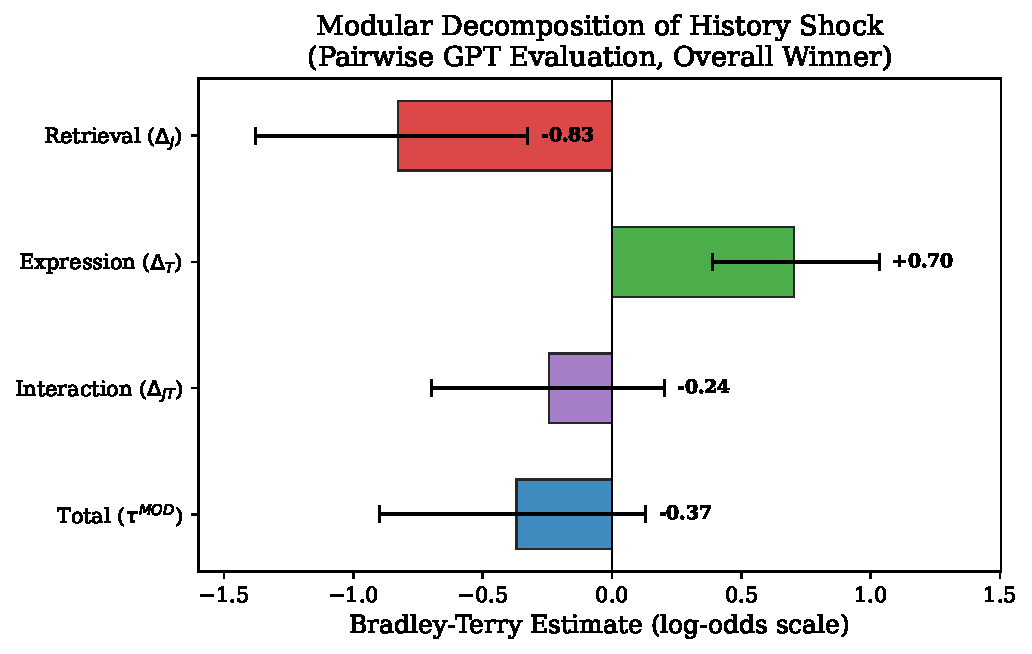
\includegraphics[width=0.85\textwidth]{figures/fig_main_decomposition.pdf}
\caption{Bradley--Terry decomposition of the history-shock effect. Each bar is a log-strength estimate; error bars show 95\% cluster-bootstrap confidence intervals. The retrieval effect ($\Delta_J$) is uniformly negative while the expression effect ($\Delta_T$) is positive for overall quality, satisfaction, and trust. The two channels nearly cancel in total.}
\label{fig:decomposition}
\end{figure}

The core finding is that the history-shock treatment has two large, opposing effects that nearly cancel in the overall synthetic evaluation. Applying the treatment to retrieval reduces evaluated recommendation quality ($\hat{\Delta}_J = -0.828$, CI excludes zero), while applying it to expression improves evaluated quality ($\hat{\Delta}_T = +0.704$, CI excludes zero). The net total effect $\hat{\tau}^{MO} = -0.369$ is negative but statistically insignificant. A standard prompt A/B test comparing cell $(0,0)$ to cell $(1,1)$ would recover only this weak total and miss the fact that two large channel effects offset each other. The interaction $\hat{\Delta}_{JT} = -0.245$ is negative but insignificant.

\subsection{Retrieval effect: premium-aspiration bias}\label{section:retrieval-mechanism}

To understand what drives the negative retrieval effect, we examine product-level changes. History-aware retrieval ($D_i^J = 1$) selects a different product than generic retrieval ($D_i^J = 0$) in 49 of 60~clusters (82\%), confirming that the retrieval treatment is not inert. Among these 49~switched clusters, the history-aware product is on average \$25 more expensive, has fewer reviews (log rating-count difference: $-0.18$), and occupies a lower popularity tier (mean rank worsens by 3.8~positions). In 27\% of switched clusters, the generic product falls within the consumer's stated budget while the history-aware product exceeds it.

Averaging across all 60~clusters, the retrieval treatment under generic expression reduces fit by 0.70~points (1--7 scale, CI excludes zero) and purchase probability by 13.8~percentage points (CI excludes zero). These magnitudes are nearly identical under history-aware expression (fit: $-0.75$; purchase: $-14.2$~pp), confirming that the retrieval harm operates through product selection, not text quality. GPT pairwise evaluations of cell~$(0,0)$ vs.\ cell~$(1,0)$ (generic wins 73\%) cite feature match (53\%), tradeoff disclosure (40\%), and budget fit (37\%) as the most frequent reasons.

We label this pattern \emph{premium-aspiration bias}. When the LLM receives segment-level satisfaction feedback --- phrases such as ``strong post-purchase feedback among travelers'' or ``frequently chosen by audiophiles'' --- it shifts away from budget-appropriate, feature-matched products toward more expensive alternatives. In this experiment, the pattern is not simple popularity bias: the history-aware model does not shift toward bestsellers but toward products that received favorable qualitative feedback, even when those products strain the consumer's stated budget constraint.

\subsection{Expression effect: trust and tradeoff disclosure}\label{section:expression-mechanism}

Whereas the retrieval channel harms outcomes through product mismatch, the positive expression effect operates through a different mechanism: trust and tradeoff disclosure, not increased persuasion. History-aware expression ($D_i^T = 1$) increases trust by 0.58~points (1--7 scale, CI excludes zero) and tradeoff disclosure by 0.97~points (CI excludes zero) under baseline retrieval. Persuasive intensity is essentially unchanged ($+0.07$, insignificant). The treatment makes the text more informative and balanced rather than more promotional.

Notably, these text-quality gains are attenuated under history-aware retrieval: trust rises by only 0.22 (vs.\ 0.58) and tradeoff disclosure by 0.37 (vs.\ 0.97). The resulting interaction effects are $-0.37$ for trust and $-0.60$ for tradeoff disclosure, both with CIs excluding zero. This pattern aligns with the trust interaction in Table~\ref{table:bt-decomposition} ($\hat{\Delta}_{JT}^{\mathrm{trust}} = -0.717$, $P(>0) = 0.4\%$): when the retrieval stage selects a poorly matched product, the expression stage's experience-based text appears less credible.

\subsection{Outcome heterogeneity}

Looking beyond the overall measure, the four outcome dimensions in Table~\ref{table:bt-decomposition} reveal distinct compositions. \emph{Purchase intent} is dominated by retrieval: $\hat{\Delta}_J^{\mathrm{purchase}} = -1.663$ is the largest component across all dimensions, while expression is negligible ($-0.096$, $P(>0) = 32\%$). Better writing does not compensate for a mismatched product when the outcome is willingness to buy. The purchase interaction is positive ($+0.426$, $P(>0) = 95.4\%$), but the corresponding absolute-evaluation interaction is near zero ($-0.4$~pp, CI $[-3.1, +2.2]$), so we do not build a mechanism claim around it. \emph{Satisfaction} follows the overall pattern (retrieval: $-0.913$; expression: $+0.649$) with a negligible interaction. \emph{Trust} has the largest expression effect ($+1.117$) and the only clearly significant interaction ($-0.717$), consistent with the diminishing-returns mechanism documented in Section~\ref{section:expression-mechanism}.

Figure~\ref{fig:cell-means} displays the $2 \times 2$ cell means across five absolute-evaluation outcomes, illustrating the opposing patterns: history-aware retrieval reduces fit and purchase probability, while history-aware expression increases trust and tradeoff disclosure.

\begin{figure}[t]
\centering
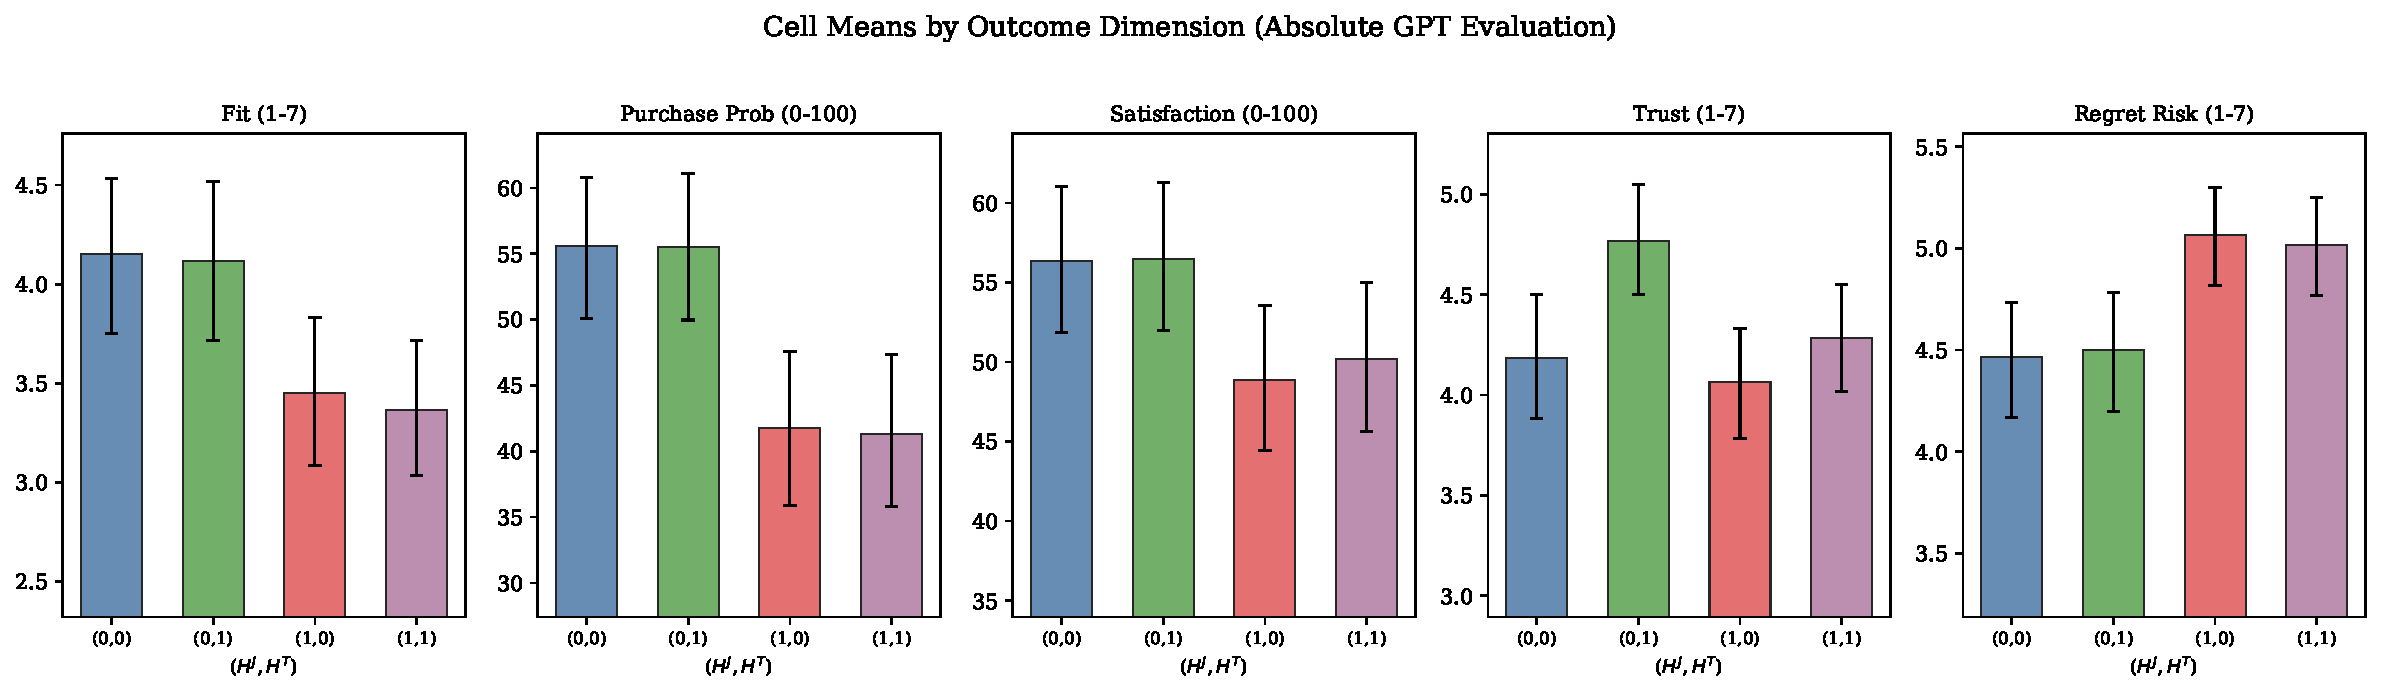
\includegraphics[width=\textwidth]{figures/fig_cell_means_outcomes.pdf}
\caption{Absolute-evaluation cell means across the $2 \times 2$ design ($n = 60$ per cell). Each panel shows the four modular cells. Moving from $D_i^J = 0$ to $D_i^J = 1$ (within columns) reduces fit and purchase probability. Moving from $D_i^T = 0$ to $D_i^T = 1$ (within rows) increases trust and tradeoff disclosure. Supplementary figures are in Appendix~\ref{section:supplementary-figures}.}
\label{fig:cell-means}
\end{figure}

\subsection{Best modular policy: generic retrieval with history-aware expression}

Table~\ref{table:pairwise-wins} reports the pairwise win-rate matrix across all six modular cell comparisons. Cell $(0,1)$ --- generic retrieval with history-aware expression --- wins the majority in every comparison: it defeats the baseline $(0,0)$ with 78\%, the full bundle $(1,1)$ with 72\%, and the retrieval-only $(1,0)$ with 73\%. No other cell achieves a win rate above 65\% in any comparison.

\begin{table}[t]
\centering
\caption{Pairwise win rates (GPT-5.3 overall evaluation, blinded, order-randomized). Each row reports $n = 60$ within-cluster comparisons. Ties: 3 of 360 total comparisons.}
\label{table:pairwise-wins}
\small
\begin{tabular}{cccccc}
\toprule
Cell A & Cell B & A wins & B wins & Ties & A win\% \\
\midrule
$(0,0)$ & $(0,1)$ & 13 & 47 & 0 & 21.7\% \\
$(0,0)$ & $(1,0)$ & 44 & 14 & 2 & 73.3\% \\
$(0,0)$ & $(1,1)$ & 39 & 21 & 0 & 65.0\% \\
$(0,1)$ & $(1,1)$ & 43 & 17 & 0 & 71.7\% \\
$(1,0)$ & $(0,1)$ & 16 & 44 & 0 & 26.7\% \\
$(1,0)$ & $(1,1)$ & 21 & 38 & 1 & 35.0\% \\
\bottomrule
\end{tabular}
\end{table}

In this controlled setting, the dominance of cell $(0,1)$ suggests that historical marketplace information is more valuable when routed to the text-generation stage---where it improves trust and disclosure---than to the retrieval stage, where it triggers premium-aspiration bias. This finding illustrates the type of architectural diagnosis the modular design enables: the same LLM and the same marketplace data are used, but the information routing between the retrieval and expression stages is changed. Whether this specific routing recommendation generalizes beyond the product category, supply model, and synthetic evaluation studied here is an empirical question that the design can answer in other settings.

\subsection{Black-box architecture comparison}\label{section:bb-diagnostic}

The modular decomposition above is identified within a two-stage system where retrieval and expression are separated by construction. A natural question is whether this separation itself changes the recommendation package --- that is, whether the modular system behaves similarly to a unified black-box recommender. To assess this, we compare each unified black-box recommendation against the corresponding modular diagonal cell via blinded pairwise GPT evaluation: unified $Z=0$ versus modular cell $(0,0)$, and unified $Z=1$ versus modular cell $(1,1)$.

Under the baseline condition, the two architectures are nearly indistinguishable. Product agreement is 83.3\% (50 of 60 clusters select the same product), and pairwise win rates are balanced: the unified recommender wins 46.7\% of overall comparisons versus 51.7\% for the modular system, with similar splits on purchase, satisfaction, and trust outcomes. No systematic quality difference is detectable.

Under the treated condition, the modular diagonal wins the synthetic pairwise comparison against the unified black-box. Product agreement drops to 61.7\%, and the modular system wins 71.7\% of overall comparisons (unified: 28.3\%). The same pattern appears across the component outcomes: purchase (56.7\% vs.\ 40.0\%), satisfaction (68.3\% vs.\ 25.0\%), and trust (71.7\% vs.\ 23.3\%).

This asymmetry has a natural interpretation. At baseline, both architectures draw on the same product specifications and generate similar recommendation packages. Under the history-access treatment, the unified system bundles retrieval and expression reasoning in a single call, while the modular system routes history to each stage with explicit control. The two-stage separation may produce better-targeted treated recommendations because the expression stage receives a locked product and can focus on communication rather than jointly reasoning about selection and language. The main decomposition results should therefore be interpreted as effects within the experimentally modularized system. The black-box comparison is reassuring because the modular system is not visibly dominated by the unified assistant in this diagnostic, but it does not prove that the decomposition fully explains every black-box LLM recommender.

%-------------------------------------------------------------------------
\section{Conclusion}\label{section:conclusion}
%-------------------------------------------------------------------------

This paper proposes a modular $2 \times 2$ experimental design that decomposes the effect of an LLM recommender policy change into a retrieval effect, an expression effect, and their interaction. The framework builds on a simple observation: LLM-mediated product recommendation bundles two economically distinct functions---product selection and explanatory language---and a standard prompt A/B test cannot tell a firm which function is responsible for the observed consumer response.

\paragraph{Summary of findings.}
In a semi-synthetic study using real headphone products and consumer personas, we find that routing historical marketplace information to the retrieval stage reduces evaluated recommendation quality, while routing the same information to the expression stage improves evaluated trust and disclosure. The two channels nearly cancel, producing an insignificant total effect---a standard A/B test would recover only this weak total and miss the opposing channel structure. A black-box comparison finds that the modular system is similar to the unified recommender at baseline and wins the synthetic pairwise comparison under the history-access treatment. This diagnostic reduces, but does not eliminate, concern that the results are driven mechanically by the two-stage architecture.

\paragraph{Managerial implications.}
The findings are relevant to e-commerce platforms, retail firms, and marketing technology providers that deploy or evaluate LLM shopping assistants. Three implications stand out.

First, \emph{prompt A/B tests are insufficient for diagnosing LLM recommenders}. A test that compares two versions of a recommender identifies the total effect of the policy change, but the total effect does not tell the firm whether to invest in better retrieval, better expression, or both. The modular design separates these channels at the cost of running four cells instead of two.

Second, \emph{information routing can matter as much as information access}. In our setting, the same historical buyer information is valuable when routed to text generation---where it improves trust and tradeoff disclosure---but harmful when routed to product selection---where it triggers premium-aspiration bias. Our results suggest that giving an LLM recommender access to marketplace data without controlling how that data enters the recommendation pipeline can inadvertently degrade product-consumer fit.

Third, \emph{realized-text regressions can misattribute product fit to expression}. A researcher who scores generated recommendations for endorsement strength and regresses outcomes on that score may partly attribute product-fit effects to language. We derive a closed-form bias that is non-monotonic in the endogeneity parameter when expression intensity positively covaries with latent product fit. The modular design avoids this problem by randomizing the expression policy before text generation.

\paragraph{Limitations and future research.}
Several limitations of the current study point to directions for future research. First, all consumer outcomes are evaluated by a separate LLM (GPT-5.3), not by human consumers. While synthetic evaluation is useful for demonstrating the decomposition methodology and generating directional findings, it does not establish how real consumers respond to LLM-generated recommendations. A natural next step is a human-subject experiment that deploys the same modular $2 \times 2$ design with real consumers evaluating recommendation packages. Such an experiment would test whether the opposing-channel pattern replicates with human judgments and whether the magnitude of the retrieval and expression effects differs from synthetic evaluation.

Second, the design identifies effects over the feasible recommendation support---products that neither retrieval policy nominates lie outside the estimand. Extending the framework to richer policy spaces with more than two retrieval conditions is a natural next step.

Third, our findings come from one product category (headphones), one supply model (Qwen~2.5~14B), and one type of information shock (history access). Whether the premium-aspiration bias generalizes to other categories, frontier models, or different policy contrasts---such as prompt engineering, fine-tuning, or retrieval-augmented generation---remains an open question. Replicating the design across product domains and LLM architectures would strengthen the external validity of the decomposition.

Fourth, we define the architecture gap $\Gamma = \tau^{BB} - \tau^{MO}$ conceptually and assess it through a qualitative pairwise diagnostic, but we do not estimate $\Gamma$ as a quantitative effect-size difference. Developing a formal estimator for the architecture gap---on a common outcome scale across the unified and modular designs---would allow researchers to test whether the modular decomposition fully accounts for the black-box treatment effect. We leave this extension for future work.

Finally, the current framework treats the retrieval and expression stages as binary policy switches. In practice, firms may want to optimize continuous policy parameters---such as how much historical information to provide or how strongly to instruct the expression stage toward transparency. Extending the framework to continuous or multi-level treatments and connecting it to optimal policy design is a promising direction for future work.

\bigskip
\bibliographystyle{plainnat}
\bibliography{references}

\newpage

\appendix

%-------------------------------------------------------------------------
\section{Analytical Derivations}\label{section:proofs}
%-------------------------------------------------------------------------

\subsection{Non-identification counterexample}\label{section:proof-nonid}

We construct a counterexample showing that the black-box total effect does not identify $\dR$, $\dP$, or $\dRP$ separately. Consider two products $\{j_1, j_2\}$ and two expression states $\{e_0, e_1\}$, and write the potential outcomes as a $2 \times 2$ matrix $\Y(\cdot, \cdot)$. Let the black-box kernels be $\KOS_0(j, e) = 0.5 \cdot \mathbf{1}\{j = j_1, e = e_0\} + 0.5 \cdot \mathbf{1}\{j = j_2, e = e_0\}$ and $\KOS_1(j, e) = 0.5 \cdot \mathbf{1}\{j = j_1, e = e_1\} + 0.5 \cdot \mathbf{1}\{j = j_2, e = e_1\}$. Then
\[
\dtotal = \tfrac{1}{2}\!\left[\Y(j_1, e_1) - \Y(j_1, e_0)\right] + \tfrac{1}{2}\!\left[\Y(j_2, e_1) - \Y(j_2, e_0)\right].
\]
Now consider two potential-outcome arrays. \textbf{Array~A} has $\Y(j_1, e_0) = 0.2$, $\Y(j_1, e_1) = 0.4$, $\Y(j_2, e_0) = 0.3$, $\Y(j_2, e_1) = 0.5$. \textbf{Array~B} has $\Y(j_1, e_0) = 0.3$, $\Y(j_1, e_1) = 0.5$, $\Y(j_2, e_0) = 0.2$, $\Y(j_2, e_1) = 0.4$. Both arrays yield $\dtotal = 0.2$, but the implied modular cell means differ: array~A and array~B generate different $(\dR, \dP, \dRP)$ triples despite producing the same $\dtotal$. $\square$

\subsection{Naive realized-expression bias}\label{section:proof-naive}

Standard omitted-variable bias for OLS. The full population regression $\Y = \beta_0 + \beta_E \E + \beta_Q \tilde{\Q} + \nu$ is correctly specified. The naive regression omits $\tilde{\Q}$, and the OLS coefficient on $\E$ satisfies
\[
\mathrm{plim}\, \hat{\beta}_E^{\mathrm{naive}} = \beta_E + \frac{\mathrm{Cov}(\E, \tilde{\Q})}{\mathrm{Var}(\E)} \beta_Q.
\]
With $\E = e_0 + \tau \Rreg + \lambda_{\mathrm{fit}} \tilde{\Q} + \sigma_E \eta$ and $\eta, \tilde{\Q}, \Rreg$ mutually independent, $\mathrm{Cov}(\E, \tilde{\Q}) = \lambda_{\mathrm{fit}} \mathrm{Var}(\tilde{\Q})$ and $\mathrm{Var}(\E) = \lambda_{\mathrm{fit}}^2 \mathrm{Var}(\tilde{\Q}) + \sigma_E^2 + \tau^2 \mathrm{Var}(\Rreg)$. Substituting yields the closed form in Equation~\eqref{eq:naive-expression-bias}. $\square$

The absolute value of the bias term is non-monotonic in $\lambda_{\mathrm{fit}}$ when $\lambda_{\mathrm{fit}}$ moves away from zero with fixed sign. Let $A = \tau^2\mathrm{Var}(\Rreg)+\sigma_E^2$ and $V_Q=\mathrm{Var}(\tilde{\Q})$. The relevant bias factor is $b(\lambda)=\lambda V_Q/(\lambda^2 V_Q + A)$. Differentiating gives $b'(\lambda)=V_Q(A-\lambda^2V_Q)/(\lambda^2V_Q+A)^2$, so the positive-side maximum occurs at $\lambda_{\mathrm{fit}}^\star=\sqrt{A/V_Q}$.

%-------------------------------------------------------------------------
\section{Monte Carlo Validation of the Estimator}\label{section:dgp}
%-------------------------------------------------------------------------

To validate that the modular design recovers known ground-truth effects under controlled conditions, we construct a structural data-generating process (DGP) with three hand-curated product catalogs (phone chargers, headphones, laptops) and 1{,}000 simulated consumers per category. Throughout this appendix, $q$ denotes the retrieval policy indicator (corresponding to $D_i^J$ in the main text), $r$ denotes the expression policy indicator ($D_i^T$), and $z$ denotes the black-box treatment ($D_i$). Each consumer-product pair has a latent fit score $\Q_{ij}$, and we simulate outcomes under two DGPs: a expression-leaning DGP (brand-forward retrieval, expression as leading channel) and a retrieval-dominant DGP (fit-aware retrieval). Under both DGPs, the modular design recovers the three components within sampling noise, while the naive realized-expression regression overstates the expression effect by 80--130\% at policy-relevant endogeneity levels. The structural validation is documented in detail below.

\subsection{Retrieval kernel}

Under the expression-leaning DGP, the retrieval score for consumer $i$ and product $j$ is
\[
\mathrm{score}_{ij}(q) = a_Q \tilde{\Q}_{ij} + a_{\mathrm{inc}} \mathrm{incumbent}_j + a_{\mathrm{focal}} \cdot q \cdot \mathrm{focal\_brand}_j + \sigma_R \varepsilon_{ij},
\]
where $\tilde{\Q}_{ij}$ is the within-category standardized fit score and $\varepsilon_{ij} \sim \mathcal{N}(0, 1)$. The selected product is $\J_i(q) = \arg\max_{j} \mathrm{score}_{ij}(q)$. Under the retrieval-dominant DGP, the $a_{\mathrm{focal}}$ term is replaced by a direct $Q$-boost: $\mathrm{score}_{ij}(q) = (a_Q + \delta_{\mathrm{fit}} \cdot q) \tilde{\Q}_{ij} + a_{\mathrm{inc}} \mathrm{incumbent}_j + \sigma_R \varepsilon_{ij}$.

\subsection{Expression kernel}

One-shot: $\E_i(z) = e_0 + \tau_{\mathrm{backend}} z + \lambda_{\mathrm{fit}} \tilde{\Q}_{i, \J_i(z)} + \lambda_{\mathrm{inc}} \mathrm{incumbent}_{\J_i(z)} + \sigma_E \eta_i$.
Modular: $\E_i(q, r) = e_0 + \tau_R r + \lambda_{\mathrm{fit}} \tilde{\Q}_{i, \J_i(q)} + \lambda_{\mathrm{inc}} \mathrm{incumbent}_{\J_i(q)} + \sigma_E \eta_i$.

\subsection{Outcome equation}

$\Y_i \sim \mathrm{Bernoulli}(\sigma(U_i))$ with $U_i = \beta_0 + \beta_Q \tilde{\Q}_{i,\J_i} + \beta_E \E_i + \beta_{\mathrm{inc}} \mathrm{incumbent}_{\J_i} + \beta_{\mathrm{incE}} \mathrm{incumbent}_{\J_i} \E_i$.

\subsection{Parameter values}

\begin{tabular}{lr@{\hskip 24pt}lr}
\toprule
\multicolumn{2}{c}{Expression-leaning DGP} & \multicolumn{2}{c}{Retrieval-dominant DGP} \\
$a_Q = 1.0$ & $a_{\mathrm{inc}} = 0.20$ & $a_Q = 1.0$ & $a_{\mathrm{inc}} = 0.20$ \\
$a_{\mathrm{focal}} = 0.50$ & $\sigma_R = 0.35$ & $a_{\mathrm{focal}} = 0$ & $\delta_{\mathrm{fit}} = 0.80$ \\
$e_0 = 0$ & $\tau_{\mathrm{backend}} = 0.50$ & $e_0 = 0$ & $\tau_{\mathrm{backend}} = 0.50$ \\
$\tau_R = 0.50$ & $\lambda_{\mathrm{fit}} = 1.0$ & $\tau_R = 0.50$ & $\lambda_{\mathrm{fit}} = 1.0$ \\
$\lambda_{\mathrm{inc}} = 0.20$ & $\sigma_E = 0.50$ & $\lambda_{\mathrm{inc}} = 0.20$ & $\sigma_E = 0.50$ \\
$\beta_0 = -0.80$ & $\beta_Q = 0.70$ & $\beta_0 = -0.80$ & $\beta_Q = 0.70$ \\
$\beta_E = 0.50$ & $\beta_{\mathrm{inc}} = 0.25$ & $\beta_E = 0.35$ & $\beta_{\mathrm{inc}} = 0.25$ \\
$\beta_{\mathrm{incE}} = -0.15$ & $\beta_{QE} = 0$ & $\beta_{\mathrm{incE}} = -0.15$ & $\beta_{QE} = 0$ \\
\bottomrule
\end{tabular}

\subsection{Validation results}

Pooled across the three categories, the modular cell contrasts recover the expression effect at $t = 2.56$ (estimate 0.032 against truth 0.037) in the expression-leaning DGP, and the retrieval effect at $t = 1.44$ (estimate 0.018 against truth 0.014) in the retrieval-dominant DGP. The naive estimator overstates the expression effect by 135\% of the truth at $\lambda_{\mathrm{fit}} = 1.0$. A Monte Carlo sweep across $\lambda_{\mathrm{fit}} \in \{0, 0.25, 0.5, 0.75, 1.0, 1.5, 2.0\}$ with 25~replications per value traces the non-monotonic bias pattern predicted by Equation~\eqref{eq:naive-expression-bias}. Master seed: 20260513 with \texttt{numpy.random.SeedSequence.spawn(5)}.

%-------------------------------------------------------------------------
\section{Pilot Implementation Check}\label{section:pilot}
%-------------------------------------------------------------------------

Before running the main study, we verified that the modular prompt architecture could generate parseable recommendations in all four cells and produce nontrivial variation in retrieval and expression. We deployed the four-cell design on a local LLM (Qwen~2.5~14B) across three product categories---phone chargers (8~products, 10~personas), headphones (10~products, 10~personas), and laptops (10~products, 10~personas)---yielding 120~recommendation packages across 30~clusters. GPT-5.3 evaluated all $\binom{4}{2} \times 30 = 180$ within-cluster pairwise comparisons under a blinded protocol. We fit a Bradley--Terry model \citep{bradley1952rank} with $\theta_{00} = 0$ as the reference and obtained confidence intervals via cluster bootstrap ($B = 2{,}000$).

\begin{center}
\small
\begin{tabular}{lrrrr}
\toprule
& \multicolumn{4}{c}{Bradley--Terry $\hat{\theta}$} \\
Category & Retrieval & Expression & Interaction & Total \\
\midrule
Headphones    & $-$0.19 & 1.21 & 0.01 & 1.03 \\
Laptops       & $-$0.16 & 0.31 & 0.54 & 0.69 \\
Phone chargers & 0.60  & 1.13 & $-$0.59 & 1.14 \\
\midrule
\textbf{Pooled} & \textbf{0.08} & \textbf{0.84} & \textbf{0.00} & \textbf{0.93} \\
\bottomrule
\end{tabular}
\end{center}

All four cells produced parseable, non-degenerate recommendations. The expression effect was large and precisely estimated in the pooled sample ($\hat{\Delta}_T = 0.84$, CI $[0.46, 1.20]$). The pooled interaction was negligible ($\hat{\Delta}_{JT} = 0.00$, $P(>0) = 51\%$). Category-level interactions had opposing signs for laptops ($+0.54$) and phone chargers ($-0.59$), consistent with noise at $n = 10$ clusters per category. We therefore use the pilot only as a feasibility check for the four-cell architecture, not as evidence for the sign or magnitude of the main experimental effects.

%-------------------------------------------------------------------------
\section{Product Catalog and Metadata}\label{section:catalog}
%-------------------------------------------------------------------------

The catalog comprises 30 headphone products selected from the Amazon Reviews 2023 dataset based on the following criteria: (i)~at least 30{,}000 customer ratings, (ii)~available price data, (iii)~brand diversity (21 unique brands). Products span four popularity tiers assigned by rating-count quartiles: bestseller (top 25\%, $\geq$100K ratings), mainstream (50--75th percentile), niche (25--50th), and long tail (bottom 25\%). Price tiers are assigned as budget ($\leq$\$25), midrange (\$26--\$100), and premium ($>$\$100), with 10 products per tier. The correlation between popularity rank and price is $+0.12$; between popularity rank and average rating, $+0.31$.

For each product, we extract: ASIN, title, brand, price, average rating, rating count, raw feature list, and description from the Amazon metadata files. We derive key features (top 4 from the raw feature list), best-for segments (inferred from feature keywords), and drawbacks (inferred from common complaint patterns in the reviews).

%-------------------------------------------------------------------------
\section{Consumer Persona Generation}\label{section:personas}
%-------------------------------------------------------------------------

We generate 60 consumer personas using GPT, with 7--8 personas per segment across 8 segments: budget student, commuter, frequent traveler, remote worker, audiophile, gym user, gamer, and casual listener. Each persona includes: a one-paragraph natural-language description, an age range, a purchase context, a budget range, a technical knowledge level (low/medium/high), a primary use case, a secondary use case, must-have features, and features to avoid. The generation prompt asks GPT to produce diverse, realistic personas that span the attribute space within each segment.

%-------------------------------------------------------------------------
\section{Prompt Templates}\label{section:prompts}
%-------------------------------------------------------------------------

This appendix reproduces the exact prompts used for each cell of the $2 \times 2$ design. All prompts are sent to Qwen~2.5~14B via Ollama at temperature 0.7.

\subsection{System prompts}

\textbf{Generic recommender persona} ($\Qreg = 0$ or $\Rreg = 0$):

\begin{quote}
\small\ttfamily
You are a product recommender. You only have access to the product catalog and the consumer's stated needs. You do NOT have access to sales data, review summaries, popularity rankings, or historical purchase feedback. Recommend based solely on product specifications and how they match the consumer's requirements.
\end{quote}

\textbf{History-aware recommender persona} ($\Qreg = 1$ or $\Rreg = 1$):

\begin{quote}
\small\ttfamily
You are an experienced shopping recommender. You have access to product attributes, public review summaries, and internal historical purchase-feedback patterns. Your goal is not to recommend the most popular product. Your goal is to recommend the product most suitable for this specific consumer. Use historical evidence as background only. Do not cite exact sales numbers, conversion rates, satisfaction rates, ranks, sample sizes, or percentages. You may refer qualitatively to evidence such as ``often chosen by similar buyers,'' ``strong post-purchase feedback among travelers,'' ``mixed feedback from budget buyers,'' or ``frequent complaints about comfort.''
\end{quote}

\subsection{Retrieval prompts}

\textbf{Generic retrieval} ($\Qreg = 0$): The LLM receives the generic persona, the consumer profile (one-paragraph description, budget, primary use case, must-have features, features to avoid), and the product catalog formatted as a list with product ID, brand, model name, price, average rating, and top 4 features. The catalog does \emph{not} include rating counts, popularity tiers, or review summaries. The prompt instructs: ``Select the single best product for this consumer based on their stated needs and the product specifications.'' Output: JSON with \texttt{selected\_product\_id} and \texttt{retrieval\_rationale\_internal}.

\textbf{History-aware retrieval} ($\Qreg = 1$): The LLM receives the history-aware persona, the same consumer profile, and the product catalog enhanced with rating counts, popularity tiers, and qualitative summaries of segment-level affinity. The prompt instructs: ``Consider both the consumer's stated needs AND which products have historically satisfied similar buyers. If a popular, well-reviewed product fits the consumer's needs, prefer it over an obscure alternative --- unless the consumer has specific requirements the popular option cannot meet.'' Output: JSON with \texttt{selected\_product\_id}, \texttt{retrieval\_rationale\_internal}, and \texttt{history\_signal\_used}.

\subsection{Expression prompts}

\textbf{Generic expression} ($\Rreg = 0$): ``Write a recommendation based ONLY on the product specifications and the consumer's needs. Do not mention popularity, reviews, or how other buyers feel --- you only have the spec sheet.'' Style: ``Write a straightforward product recommendation based on the product specs and the consumer's stated needs. Be factual and concise. Stick to what is listed in the product features.'' Output: JSON with \texttt{recommendation\_text} (3--5 sentences), \texttt{tradeoff\_text} (1--2 sentences), and \texttt{persuasion\_text} (1 sentence).

\textbf{History-aware expression} ($\Rreg = 1$): ``Write a recommendation that naturally weaves in your knowledge of how this product performs in the real world. Reference patterns like `buyers in your situation tend to...' or `this is a proven choice for...' or `the main complaint from similar users is...' --- but NEVER cite specific numbers, percentages, or rankings.'' Style: ``Write like an experienced shopping advisor who has seen thousands of customers buy and return products. Be opinionated and specific. Use your historical insight to give advice that goes beyond the spec sheet.'' The product detail block includes historical intelligence (segment-level affinity, review snippets). Output: JSON with the same fields plus \texttt{history\_language\_used}.

%-------------------------------------------------------------------------
\section{Leakage Audit}\label{section:leakage}
%-------------------------------------------------------------------------

The leakage audit scans all recommendation packages for 18 forbidden regex patterns covering: percentages (\texttt{\textbackslash d+\%}, \texttt{\textbackslash d+\textbackslash.\textbackslash d+\%}), ordinal rankings (``ranked \#\textbackslash d+'', ``top \textbackslash d+''), specific counts (``\textbackslash d+,\textbackslash d+ reviews'', ``\textbackslash d+,\textbackslash d+ ratings''), satisfaction rates (``\textbackslash d+ out of \textbackslash d+''), sample sizes (``based on \textbackslash d+ customers''), and conversion language (``\textbackslash d+\% of buyers'', ``\textbackslash d+\% satisfaction''). Packages that trigger any pattern are regenerated with a reinforced anti-leakage instruction prepended to the prompt.

%-------------------------------------------------------------------------
\section{Estimator Details}\label{section:estimators}
%-------------------------------------------------------------------------

\subsection{Cell-mean contrasts and analytical standard errors}

For each modular cell $(q, r) \in \{0, 1\}^2$ we compute the cell mean $\bar{\Y}_{q, r}$ and the cell variance $s^2_{q, r}$. The standard error of a two-cell contrast is $\sqrt{s^2_{q_1, r_1} / n_{q_1, r_1} + s^2_{q_2, r_2} / n_{q_2, r_2}}$. The standard error of the four-cell interaction contrast is $\sqrt{\sum_{(q, r)} s^2_{q, r} / n_{q, r}}$.

\subsection{Bradley--Terry model}

We fit a Bradley--Terry model to the pairwise comparison data, treating ties as half-win/half-loss. The log-likelihood is maximized numerically with $\theta_{00} = 0$ as the identified baseline. Decomposition effects are computed as linear combinations of the four cell parameters.

\subsection{Cluster bootstrap}

We sample consumer clusters with replacement ($B = 2{,}000$) and re-estimate the Bradley--Terry model on each bootstrap sample. The $\alpha/2$ and $1 - \alpha/2$ quantiles of the bootstrap distribution provide confidence intervals. The posterior probability $P(>0)$ is the fraction of bootstrap replicates in which the effect estimate is positive.

%-------------------------------------------------------------------------
\section{Supplementary Figures for the History-Shock Experiment}\label{section:supplementary-figures}
%-------------------------------------------------------------------------

Figures~\ref{fig:pairwise-matrix}--\ref{fig:purchase-interaction} provide supplementary diagnostic visualizations for the history-shock experiment discussed in Section~\ref{section:results}.

\begin{figure}[h]
\centering
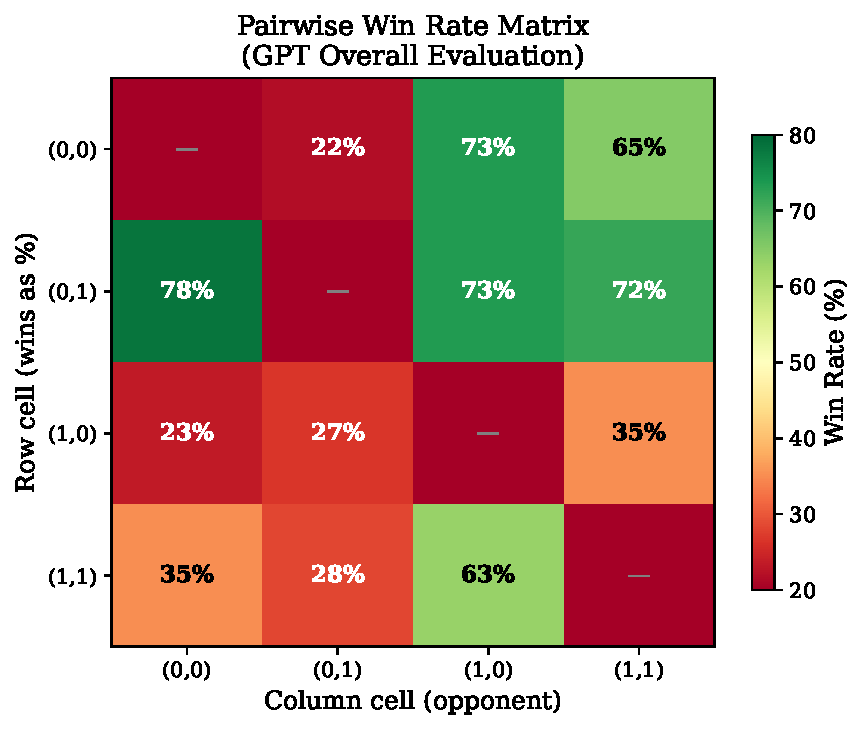
\includegraphics[width=0.7\textwidth]{figures/fig_pairwise_win_matrix.pdf}
\caption{Pairwise win-rate matrix across the four modular cells, evaluated on the overall dimension by GPT-5.3. Cell $(0,1)$ dominates all other cells.}
\label{fig:pairwise-matrix}
\end{figure}

\begin{figure}[h]
\centering
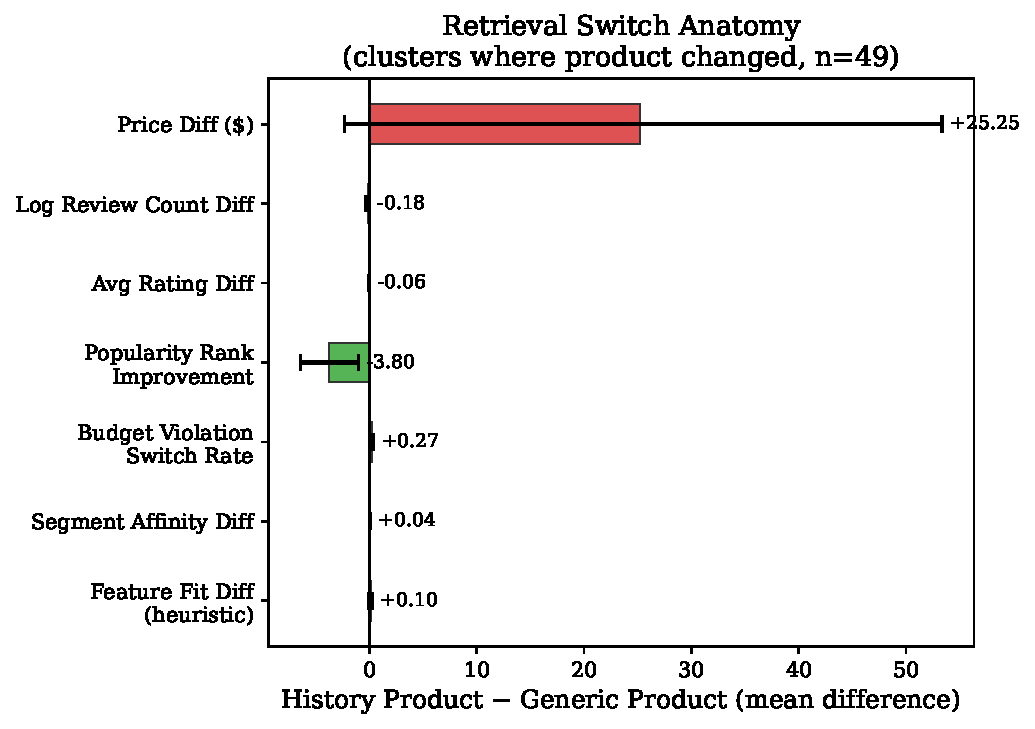
\includegraphics[width=0.85\textwidth]{figures/fig_retrieval_switch_anatomy.pdf}
\caption{Anatomy of product switches under history-aware retrieval. Among the 49~clusters where the product changes, the figure shows differences in price, log rating count, average rating, and popularity tier between the history-aware and generic product selections.}
\label{fig:retrieval-anatomy}
\end{figure}

\begin{figure}[h]
\centering
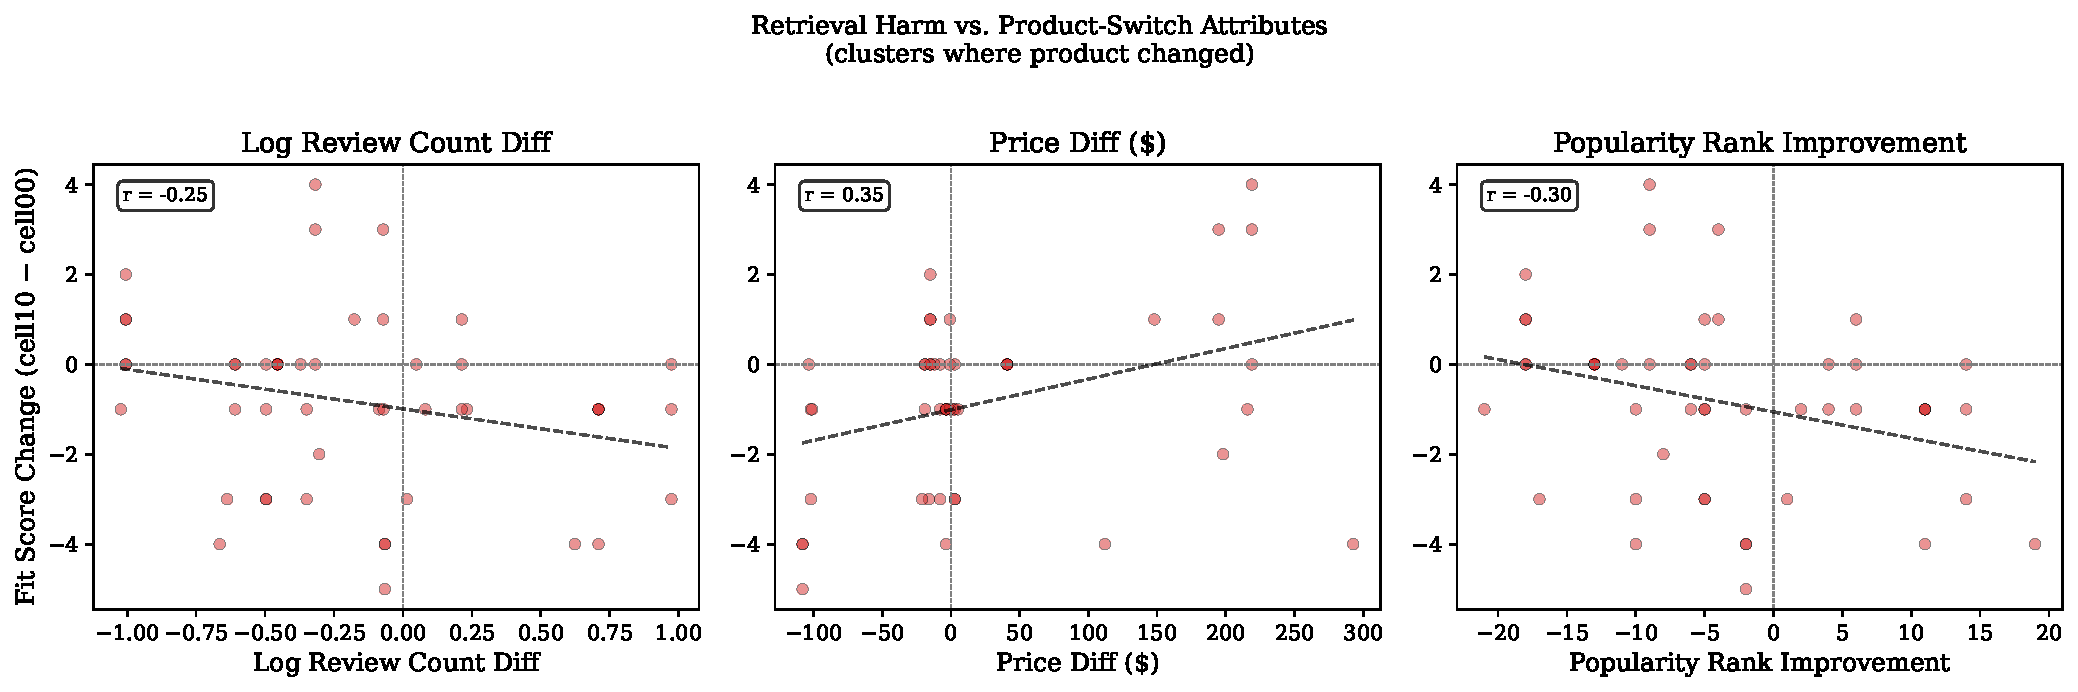
\includegraphics[width=0.85\textwidth]{figures/fig_retrieval_harm_scatter.pdf}
\caption{Cluster-level relationship between product-attribute shifts under history-aware retrieval and the resulting changes in fit score and purchase probability.}
\label{fig:retrieval-scatter}
\end{figure}

\begin{figure}[h]
\centering
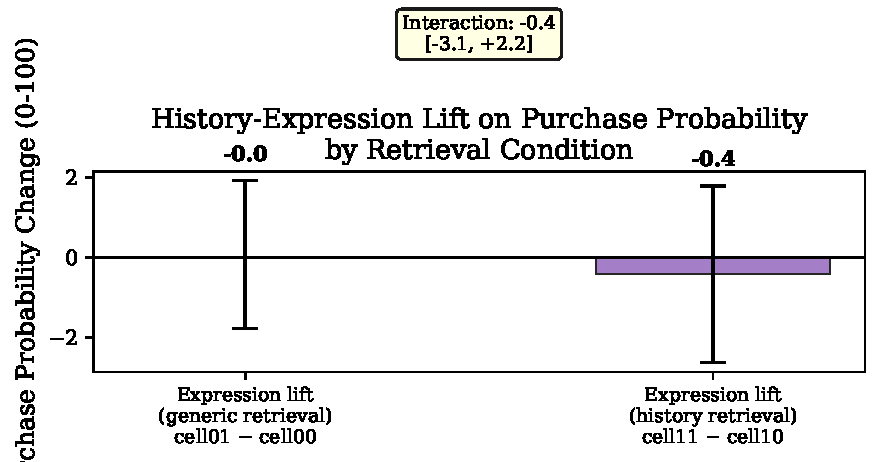
\includegraphics[width=0.85\textwidth]{figures/fig_purchase_interaction.pdf}
\caption{Expression-induced lift in purchase evaluation by retrieval condition: generic retrieval (left) vs.\ history-aware retrieval (right).}
\label{fig:purchase-interaction}
\end{figure}

\end{document}
